\chapter{Нейтронно-физический расчет ядерного реактора}

\section{Формирование активной зоны реактора}

Активная зона проектируемого реактора имеет кассетную структуру. Кассеты
имеют форму шестигранников, внутри которых находятся тепловыделяющие
элементы. Активная зона реактора тепловой мощностью 128.53 МВт (глава 2)
состоит из 121 ТВС, описанный диаметр -- 1200 мм, высота -- 1300 мм.

\begin{figure}[!h]
\center
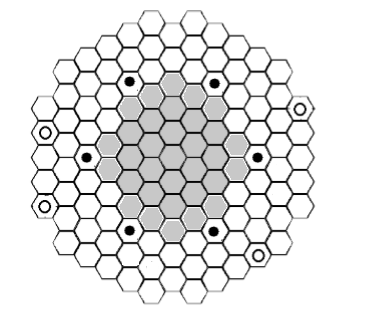
\includegraphics[width=4.43750in,height=3.83293in]{media/image12.png}
\caption{Компоновка активной зоны : - ТВС центральной зоны; - ТВС
периферийной зоны; - ТВС со стержнем АЗ; - ТВС с пустым каналом}
\end{figure}

Таблица 3.1 - Типы и состав ТВС активной зоны


\begin{longtable}[]{@{}lllll@{}}
\toprule
Тип ТВС & Число ТВС & Число "тяжелых" / "легких" твэлов & Число СВП-1 &
Число СВП-2\tabularnewline
\midrule
\endhead
ТВС центральной зоны & 33 & 69 / - & 9 & 6\tabularnewline
ТВС периферийной зоны & 78 & 18 / 51 & 9 & 6\tabularnewline
ТВС со стержнем АЗ & 6 & 18 / 51 & 9 & 6\tabularnewline
ТВС с пустым каналом & 4 & 18 / 51 & 9 & 6\tabularnewline
\bottomrule
\end{longtable}

\begin{figure}[!h]
\center
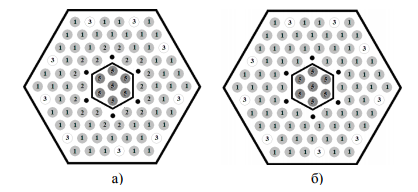
\includegraphics[width=4.59375in,height=2.10972in]{media/image13.png}
\caption{Схема размещения элементов в ТВС периферийной (а) и
центральной (б) зоны: 1 -- «тяжелые» твэлы; 2 -- «легкие» твэлы; 3 --
СВП-1; 4 -- СВП-2; 5 -- пэлы}
\end{figure}

\begin{figure}[!h]
\center
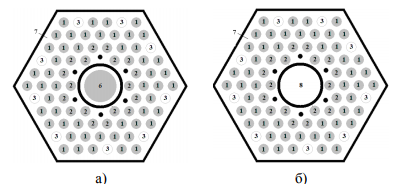
\includegraphics[width=4.15625in,height=2.00000in]{media/image14.png}
\caption{Схема размещения элементов в ТВС со стержнем АЗ (а) и
пустым каналом (б): 1 -- «тяжелые» твэлы; 2 -- «легкие» твэлы; 3 --
СВП-1; 4 -- СВП-2; 6 -- стержень АЗ; 7 -- теплоноситель; 8 -- пустой
канал}
\end{figure}

\section{Подготовка макроскопических параметров для стационарного и
динамических расчетов}


Для последующих НФР расчетов необходимо знать двухгрупповые
макроскопические параметры для каждого типа ТВС. Для твэлов с подвижными
элементами (пэлы, стержни АЗ) необходимо знать два набора
макроскопических параметров -- с поднятыми и опущенными стержнями.

Расчет данных параметров производится по спектральной программе GETERA с
использованием полиячейки (ТВС), каждый отдельный элемент (моноячейка)
-- многозонная ячейка. Для описания полиячейки необходимо знать позонную
концентрацию нуклидов, число ячеек и матрицу вероятнойстей перехода
нейтронов между отдельными моноячейками, а также температуры зон ячеек.

Для расчета концентрации нуклидов применим следующую формулу:

\(\rho_{i} = \varepsilon_{i}N_{A}\frac{\gamma_{i}}{M_{r}^{i}}\) ,

где \(N_{A}\) -- число Авогадро, \(M_{r}^{i}\) -- молярная масса,
\(\varepsilon_{i}\) -- объемная доля, \(\gamma_{i}\) -- плотность
вещества.

Применим следующие допущения:

\begin{enumerate}
\item
  Не будем учитывать наличие в материалах элементов с малой
  концентрацией или изотопов, обладающих малым макроскопическим сечением
  взаимодействия с нейтронами.
\item
  Будем считать, что температура одинакова в пределах одной зоны.
\item
  Не будем учитывать влияние компенсатора распухания и материал чехла
  ТВС на расчеты.
\end{enumerate}

\begin{quote}
Исходя из вышеперечисленных предположений, получим ядерные концентрации,
представленные в таблице 3.2

Таблица 3.2 -- Концентрация веществ, содержащихся в АЗ
\end{quote}

\begin{longtable}[]{@{}l@{}}
\toprule
ТВЭЛ-Т\tabularnewline
\midrule
\endhead
Нуклид\tabularnewline
Th\textsuperscript{232}\tabularnewline
U\textsuperscript{233}\tabularnewline
O\tabularnewline
ТВЭЛ-Л\tabularnewline
Нуклид\tabularnewline
Th\textsuperscript{232}\tabularnewline
U\textsuperscript{233}\tabularnewline
O\tabularnewline
Оболочка ТВЭЛа, СВП, ПЭЛа (сплав Э-110)\tabularnewline
Нуклид\tabularnewline
Zr\tabularnewline
Силуминовая матрица\tabularnewline
Нуклид\tabularnewline
Al\tabularnewline
Si\tabularnewline
\bottomrule
\end{longtable}

\begin{longtable}[]{@{}l@{}}
\toprule
СВП\tabularnewline
\midrule
\endhead
Нуклид\tabularnewline
Gd\textsuperscript{155}\tabularnewline
Gd\textsuperscript{157}\tabularnewline
O\tabularnewline
Al\tabularnewline
Сердечник АЗ\tabularnewline
Поглотитель\tabularnewline
Нуклид\tabularnewline
B\textsuperscript{10}\tabularnewline
B\textsuperscript{11}\tabularnewline
C\tabularnewline
Оболочка\tabularnewline
Нуклид\tabularnewline
Ni\tabularnewline
Cr\tabularnewline
Воздух\tabularnewline
Нуклид\tabularnewline
N\tabularnewline
O\tabularnewline
Сердечник ПЭЛа\tabularnewline
Нуклид\tabularnewline
B\textsuperscript{10}\tabularnewline
B\textsuperscript{11}\tabularnewline
C\tabularnewline
\bottomrule
\end{longtable}

Далее для программы GETERA необходимо рассчитать матрицу перетечки между
моноячейками :

\(P_{ij} = \frac{S_{ij}}{S_{i}}\),

где \(P_{ij}\) -- вероятность перехода нейтрона из ячейки
\emph{i} в ячейку \emph{j}, \(S_{ij}\) -- площадь поверхности,
смежной между обоими типами поверхности, \(S_{i}\) -- площадь
поверхности ячеек типа \emph{i}. Была рассчитана матрица вероятностей
(таблица 3.3).

Таблица 3.3 -- матрица вероятностей для P\emph{\textsubscript{ij}} ТВС

\begin{longtable}[]{@{}ll@{}}
\toprule
Тип ячейки & P\emph{\textsubscript{ij}}\tabularnewline
\midrule
\endhead
& ТВЭЛ-1\tabularnewline
ТВЭЛ-1 & 0.5359\tabularnewline
ТВЭЛ-2 & 0.2963\tabularnewline
СВП-1 & 0.8148\tabularnewline
СВП-2 & 0.0000\tabularnewline
ПЭЛ/АЗ & 0.0000\tabularnewline
КМ & 0.4783\tabularnewline
\bottomrule
\end{longtable}

\section{Уточнение теплофизического расчета}

После получения в программе GETERA всех необходимых макропараметров
подставим их в программу SKETCH. Она позволяет получить данные о
распределении нейтронного поля и энерговыделения в активной зоне на
начало кампании реактора. Так же из данной программы находим новое
распределение коэффициентов неравномерности по высоте
(\emph{k\textsubscript{z}}) и по радиусу (\emph{k\textsubscript{r­}}). С
данными коэффициентами пересчитываем теплофизический расчет и получаем
новое распределение теплового потока и температур по высоте. Далее
заново делаем расчет по программе GETERA c новыми полученными
температурами. Данную процедуру делаем до тех пор, пока коэффициенты
неравномерности не перестанут меняться. В данном случае количество
итераций получилось равное двум.

На графиках 3.3 и 3.4 показано окончательное распределение плотности
теплового потока и температур в ТВСМ по высоте соответственно.

\begin{figure}[!h]
\center
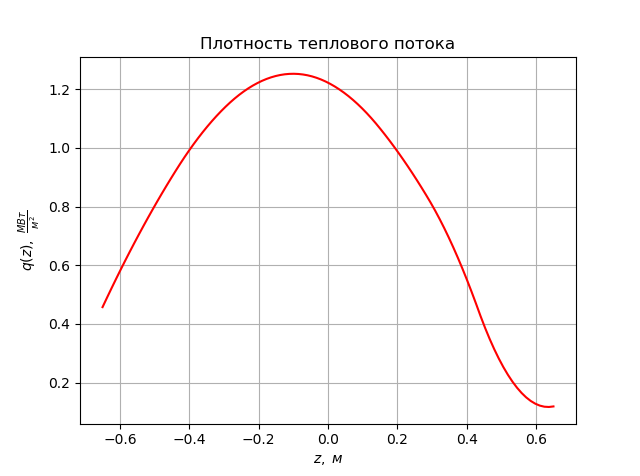
\includegraphics[width=5.11811in,height=3.80659in]{media/image15.png}
\caption{График распределения плотности теплового потока по высоте
для ТВСМ}
\end{figure}

\begin{figure}[!h]
\center
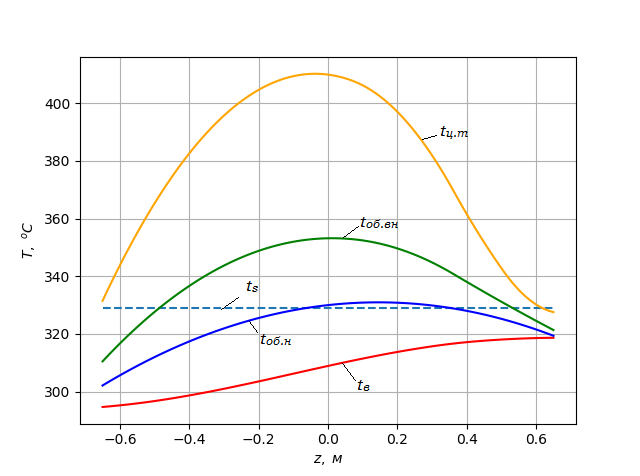
\includegraphics[width=5.11811in,height=3.80712in]{media/image16.png}
\caption{График распределения температур по высоте для ТВСМ}
\end{figure}

Таблица 3.4 -- Максимальные температуры В ТВСМ

\begin{longtable}[]{@{}ll@{}}
\toprule
& t\textsubscript{max,} $^\circ C$.\tabularnewline
\midrule
\endhead
t\textsubscript{об.н} & 331.66\tabularnewline
t\textsubscript{об.вн} & 353.83\tabularnewline
t\textsubscript{ц.т} & 420.05\tabularnewline
\bottomrule
\end{longtable}

\section{Расчет длительности кампании и выгорания топлива}

Для расчета длительности кампании была сформирована полиячейка,
состоящая из ТВС центральной и периферийной сборок. С помощью программы
GETERA было рассчитано максимальное выгорание топлива и длительность
кампании реактора (рисунок 3.5 и рисунок 3.6 соответственно).

\begin{figure}[!h]
\center
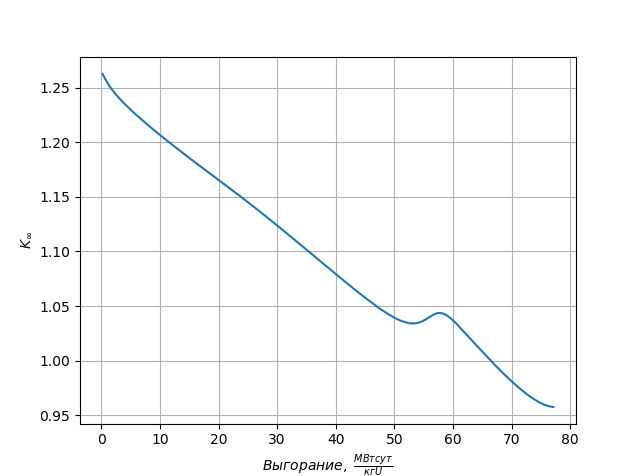
\includegraphics[width=5.11811in,height=3.80659in]{media/image17.png}
\caption{График зависимость \emph{$k_\infty$} от выгорания}
\end{figure}

\begin{figure}[!h]
\center
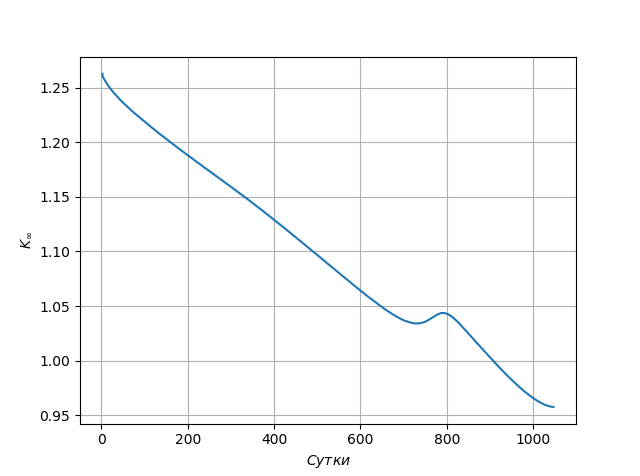
\includegraphics[width=5.11811in,height=3.80659in]{media/image18.png}
\caption{График зависимость \emph{$k_\infty$} от
количества суток}
\end{figure}

Как видно из данных графиков длительность кампании реактора $\approx$ 900 суток,
а максимальное выгорание топлива составляет
66.3\(\ \frac{MVt \cdot sut}{kg\ U}\).
